\chapter{Fíguras y otros entornos}
\label{chap:figuras}
En éste capítulo hay ejemplos de como poner figuras.
La manera mas común es que las figuras aparezcan centrados junto con su pie de figura.
 
\begin{figure}[htb]
  \centering
  \label{fig:normalDist}
  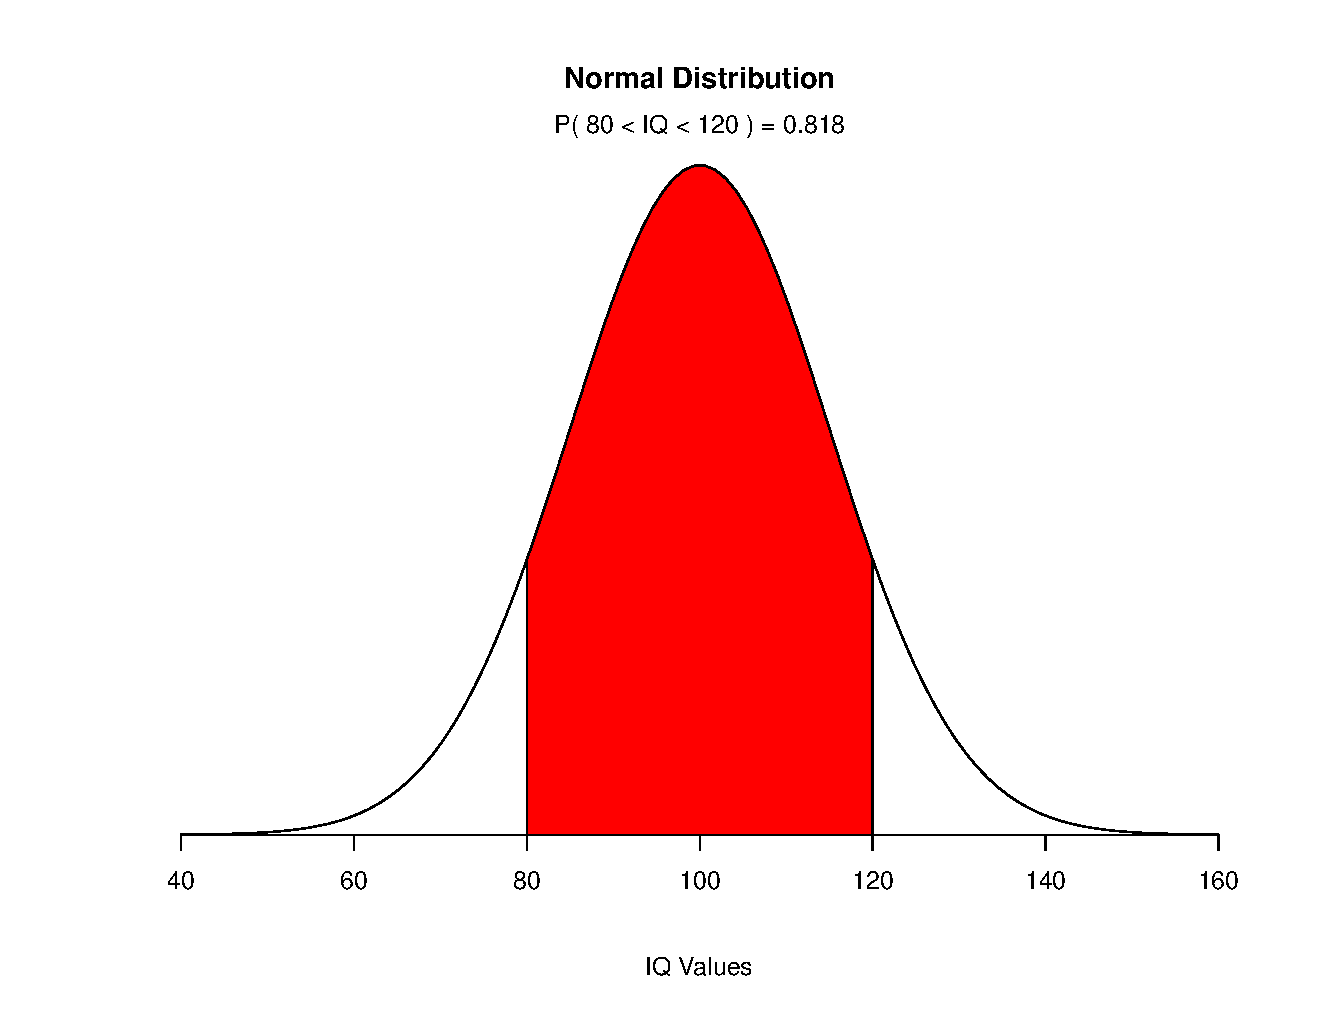
\includegraphics[width=0.85\textwidth]{img/cap02/normal}
  \caption[Distribución normal]{Gráfica de una distribución normal. Fue creado usando el siguiente \href{https://www.statmethods.net/advgraphs/probability.html}{script en R}.}
\end{figure}

\section{Subfiguras}

También es posible poner figuras, compuestas de varias subfiguras.
Cada subfigura tiene su propio pié y hay un pié de fígura extra para todo el grupo.
Posteriomente, es posible referirte e toda la fígura así: Vease la  Fígura~\ref{fig:two} ó referirte a una subfigura así:
Vea la Sub Fígura~\ref{fig:2b}.

\begin{figure}[htp]
 \centering
 \begin{subfigure}[b]{0.45\textwidth}
   \includegraphics[width=\textwidth]{img/cap02/ambiente}
   \caption{Componente de reflexión ambiental.}
 \label{fig:2a}
 \end{subfigure}
~
 \begin{subfigure}[b]{0.45\textwidth}
   \includegraphics[width=\textwidth]{img/cap02/especular}
   \caption{Componente de reflexión especular.}
   \label{fig:2b}
 \end{subfigure}
\\
 \begin{subfigure}[b]{0.45\textwidth}
   \includegraphics[width=\textwidth]{img/cap02/difuso}
   \caption{Componente de reflexión difuso.}
   \label{fig:2c}
 \end{subfigure}
~
 \begin{subfigure}[b]{0.45\textwidth}
   \includegraphics[width=\textwidth]{img/cap02/completo}
   \caption{Módelo completo.}
   \label{fig:2d}
 \end{subfigure}
 \caption[Módelo de iluminación de Phong]{Componentes del módelo de iluminación de Phong.}
 \label{fig:two}
\end{figure}

Así es como se cita un libro: éste ejemplo fué tomado de~\cite{Gonzalez:ImagenesDigitales}. 
Tambén hay un ejemplo de como hacer que un libro aparezca en las referencias sin que este citado explicitamnet en el texto. 
Por último, este es un ejemplo de una tabla muy elegante: Table \ref{tab:exey}

\begin{table}[htb]
  \begin{center}
    \begin{tabular}{l | r r r r r}
      \toprule
      Source & \textbf{DF} & \textbf{SS} & \textbf{MS} & \textbf{F} & \textbf{P-value} \\
      \midrule
      \textbf{Modelo} & 2 & 0.00318564 & 0.00159282 & 7.72 & 0.0014 \\
      \textbf{Error} & 42 & 0.00866760 & 0.00020637 &  & \\
      \midrule
      \textbf{Total} & 44 & 0.01185324 &   &  & \\
      \bottomrule
    \end{tabular}
  \end{center}
\caption{Tabla Anova para un ejercicio imaginario}
\label{tab:exey}
\end{table}
